% Editable source for fig:extension. Rebuild with make in this directory.
\documentclass[12pt,border=0pt]{standalone}
\usepackage{times,amsmath,amssymb,tikz,pgfplots}
\pgfplotsset{compat=1.18}
\newcommand{\K}{\mathcal K}
\newcommand{\eps}{\varepsilon}

\begin{document}
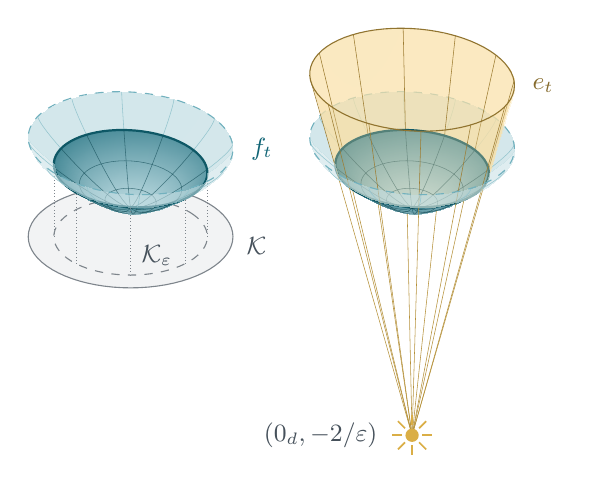
\begin{tikzpicture}[font=\small]
    \definecolor{onsloss}{HTML}{46515B}
    \definecolor{onssmooth}{HTML}{147D92}
    \definecolor{onslight}{HTML}{F2C14E}
    % K is the unit disc and eps=1/4, so K_eps is the disc of radius 3/4.
    % Both panels use the same scale for f. The yellow part is schematic:
    % the light is raised from its true height -2/eps=-8 to -\lightdepth,
    % and the rays still pass through the unchanged boundary graph of f.
    % f = (g-m)/(1-m) with
    %   g(x)=0.65 (sqrt(|x|^2+1/16)-1/4)/(sqrt(17)/4-1/4)
    %        +0.2 (1-sqrt(1-|x|^2))+0.075 (1+<w,x>),
    % where w is the unit vector at angle 145 degrees and m=0.074202 is the
    % minimum of g (computed numerically). So f is convex, f(K)=[0,1], f=1 only
    % at w, and f rises to about 0.56 on the boundary of K_eps.
    % In polar coordinates with |x|=sin(p), fp(p,t) is f; fr(r,t) is f with |x|=r.
    % fc(t) is f on the boundary of K_eps, and er(r,t) gives the schematic
    % height of the extension at distance r>=3/4 from the origin.
    % The left panel draws K at height \zf, below the graph of f.
    \def\lightdepth{3.2}
    \pgfplotsset{
        extview/.style={
                x={({\viewunit*cos(\az)},{-\viewunit*sin(\az)*sin(\el)})},
                y={({\viewunit*sin(\az)},{\viewunit*cos(\az)*sin(\el)})},
                z={(0,{0.8*\viewunit*cos(\el)})},
                axis lines=none,
                clip=false,
                anchor=origin,
                declare function={
                        fr(\r,\t)=(0.65*(sqrt(\r*\r+0.0625)-0.25)/0.780776+0.2*(1-sqrt(max(0,1-\r*\r)))+0.075*(1+\r*cos(\t-145))-0.074202)/0.925798;
                        fp(\p,\t)=fr(sin(\p),\t);
                        fc(\t)=fr(0.75,\t);
                        er(\r,\t)=(\r/0.75)*fc(\t)+\lightdepth*(\r/0.75-1);
                    },
                colormap={bowl}{color(0)=(onssmooth!30!white) color(1)=(onssmooth!80!black)},
                colormap={cut}{color(0)=(onssmooth!8!white) color(1)=(onssmooth!25!white)},
                colormap={lit}{color(0)=(onslight!15!white) color(1)=(onslight!50!white)},
                every axis plot/.append style={samples=8, samples y=48},
            },
    }
    \pgfmathsetmacro{\az}{-35}
    \pgfmathsetmacro{\el}{30}
    \pgfmathsetmacro{\pc}{asin(0.75)}
    \pgfmathsetmacro{\zf}{-0.4}
    \def\viewunit{1.3cm}

    %%%%%%%%%%%%%%%% left: f on K and the cut at K_eps %%%%%%%%%%%%%%%%
    \begin{axis}[extview, at={(0,0)}]

        % the domain K, drawn below the graph of f, with K_eps dashed
        \addplot3[fill=onsloss!7, draw=onsloss!70, thin, domain=0:360, samples=73, samples y=1]
        ({cos(x)}, {sin(x)}, \zf);
        \addplot3[onsloss!70, thin, dashed, domain=0:360, samples=73, samples y=1]
        ({0.75*cos(x)}, {0.75*sin(x)}, \zf);

        % back half of the graph of f over K minus K_eps
        \addplot3[
            surf, shader=interp, colormap name=cut, opacity=0.75,
            domain=\pc:90, y domain=\az:\az+180, samples=12,
            point meta={cos(y-\az-60)},
        ] ({sin(x)*cos(y)}, {sin(x)*sin(y)}, {fp(x,y)});
        \pgfplotsinvokeforeach{0,30,...,330}{
            \pgfmathsetmacro{\side}{sin(#1-\az)}
            \ifdim\side pt>0pt
                \addplot3[onssmooth!45, very thin, domain=\pc:90, samples=12, samples y=1]
                ({sin(x)*cos(#1)}, {sin(x)*sin(#1)}, {fp(x,#1)});
            \fi
        }

        % graph of f over K_eps
        \addplot3[
            surf, shader=interp, colormap name=bowl, z buffer=sort,
            domain=0:0.75, y domain=0:360, samples=16,
            point meta=z,
        ] ({x*cos(y)}, {x*sin(y)}, {fr(x,y)});
        \pgfplotsinvokeforeach{0,30,...,330}{
            \addplot3[onssmooth!55!black, very thin, opacity=0.6, domain=0:0.75, samples=12, samples y=1]
            ({x*cos(#1)}, {x*sin(#1)}, {fr(x,#1)});
        }
        \pgfplotsinvokeforeach{0.25,0.5}{
            \addplot3[onssmooth!55!black, very thin, opacity=0.6, domain=0:360, samples=48, samples y=1]
            ({#1*cos(x)}, {#1*sin(x)}, {fr(#1,x)});
        }

        % vertical lines from the cut down to the boundary of K_eps
        \pgfplotsinvokeforeach{-35,145,190,235,280}{
            \addplot3[onsloss!70, very thin, densely dotted, domain=0:1, samples=2, samples y=1]
            ({0.75*cos(#1)}, {0.75*sin(#1)}, {\zf+x*(fc(#1)-\zf)});
        }

        % graph of f over the boundary of K_eps
        \addplot3[onssmooth!70!black, thick, domain=0:360, samples=72, samples y=1]
        ({0.75*cos(x)}, {0.75*sin(x)}, {fc(x)});

        % front half of the graph of f over K minus K_eps
        \addplot3[
            surf, shader=interp, colormap name=cut, opacity=0.55,
            domain=\pc:90, y domain=\az+180:\az+360, samples=12,
            point meta={cos(y-\az-60)},
        ] ({sin(x)*cos(y)}, {sin(x)*sin(y)}, {fp(x,y)});
        \pgfplotsinvokeforeach{0,30,...,330}{
            \pgfmathsetmacro{\side}{sin(#1-\az)}
            \ifdim\side pt>0pt\else
                \addplot3[onssmooth!45, very thin, domain=\pc:90, samples=12, samples y=1]
                ({sin(x)*cos(#1)}, {sin(x)*sin(#1)}, {fp(x,#1)});
            \fi
        }

        % graph of f over the boundary of K
        \addplot3[onssmooth!60, thin, dashed, domain=0:360, samples=96, samples y=1]
        ({cos(x)}, {sin(x)}, {fp(90,x)});

        \coordinate (Af) at (axis cs:{cos(-35)},{sin(-35)},{fp(90,-35)});
        \coordinate (AK) at (axis cs:{cos(315)},{sin(315)},\zf);
        \coordinate (AKe) at (axis cs:{0.45*cos(270)},{0.45*sin(270)},\zf);
    \end{axis}
    \node[right=3pt, text=onssmooth!80!black] at (Af) {$f_t$};
    \node[right=2pt, text=onsloss] at (AK) {$\K$};
    \node[text=onsloss] at (AKe) {$\K_\eps$};

    %%%%%%%%%%%%%%%% right: the light at (0_d,-2/eps) and e %%%%%%%%%%%%%%%%
    \begin{axis}[extview, at={({2.75*\viewunit},0)}]

        % back half of the graph of f over K minus K_eps, behind the graph of e
        \addplot3[
            surf, shader=interp, colormap name=cut, opacity=0.75,
            domain=\pc:90, y domain=\az:\az+180, samples=12,
            point meta={cos(y-\az-60)},
        ] ({sin(x)*cos(y)}, {sin(x)*sin(y)}, {fp(x,y)});
        \pgfplotsinvokeforeach{0,30,...,330}{
            \pgfmathsetmacro{\side}{sin(#1-\az)}
            \ifdim\side pt>0pt
                \addplot3[onssmooth!45, very thin, domain=\pc:90, samples=12, samples y=1]
                ({sin(x)*cos(#1)}, {sin(x)*sin(#1)}, {fp(x,#1)});
            \fi
        }
        \addplot3[onssmooth!60, thin, dashed, domain=\az:\az+180, samples=48, samples y=1]
        ({cos(x)}, {sin(x)}, {fp(90,x)});

        % back half of the graph of e outside K_eps
        \addplot3[
            surf, shader=interp, colormap name=lit, opacity=0.7,
            domain=0.75:1, y domain=\az:\az+180,
            point meta={cos(y-\az-60)},
        ] ({x*cos(y)}, {x*sin(y)}, {er(x,y)});

        % rays behind the graph of f
        \pgfplotsinvokeforeach{0,30,...,330}{
            \pgfmathsetmacro{\side}{sin(#1-\az)}
            \ifdim\side pt>0pt
                \addplot3[onslight!75!black, very thin, domain=0:1, samples=2, samples y=1]
                ({0.75*x*cos(#1)}, {0.75*x*sin(#1)}, {-\lightdepth+x*(fc(#1)+\lightdepth)});
                \addplot3[onslight!65!black, very thin, domain=0.75:1, samples=2, samples y=1]
                ({x*cos(#1)}, {x*sin(#1)}, {er(x,#1)});
            \fi
        }

        % graph of e over K_eps, which is the graph of f there
        \addplot3[
            surf, shader=interp, colormap name=bowl, z buffer=sort,
            domain=0:0.75, y domain=0:360, samples=16,
            point meta=z,
        ] ({x*cos(y)}, {x*sin(y)}, {fr(x,y)});
        \pgfplotsinvokeforeach{0,30,...,330}{
            \addplot3[onssmooth!55!black, very thin, opacity=0.6, domain=0:0.75, samples=12, samples y=1]
            ({x*cos(#1)}, {x*sin(#1)}, {fr(x,#1)});
        }
        \pgfplotsinvokeforeach{0.25,0.5}{
            \addplot3[onssmooth!55!black, very thin, opacity=0.6, domain=0:360, samples=48, samples y=1]
            ({#1*cos(x)}, {#1*sin(x)}, {fr(#1,x)});
        }
        \addplot3[onssmooth!70!black, thick, domain=0:360, samples=72, samples y=1]
        ({0.75*cos(x)}, {0.75*sin(x)}, {fc(x)});

        % front half of the graph of e outside K_eps
        \addplot3[
            surf, shader=interp, colormap name=lit, opacity=0.3,
            domain=0.75:1, y domain=\az+180:\az+360,
            point meta={cos(y-\az-60)},
        ] ({x*cos(y)}, {x*sin(y)}, {er(x,y)});

        % rays in front of the graph of f
        \pgfplotsinvokeforeach{0,30,...,330}{
            \pgfmathsetmacro{\side}{sin(#1-\az)}
            \ifdim\side pt>0pt\else
                \addplot3[onslight!75!black, very thin, domain=0:1, samples=2, samples y=1]
                ({0.75*x*cos(#1)}, {0.75*x*sin(#1)}, {-\lightdepth+x*(fc(#1)+\lightdepth)});
                \addplot3[onslight!65!black, very thin, domain=0.75:1, samples=2, samples y=1]
                ({x*cos(#1)}, {x*sin(#1)}, {er(x,#1)});
            \fi
        }

        % front half of the graph of f over K minus K_eps, in front of the graph of e
        \addplot3[
            surf, shader=interp, colormap name=cut, opacity=0.55,
            domain=\pc:90, y domain=\az+180:\az+360, samples=12,
            point meta={cos(y-\az-60)},
        ] ({sin(x)*cos(y)}, {sin(x)*sin(y)}, {fp(x,y)});
        \pgfplotsinvokeforeach{0,30,...,330}{
            \pgfmathsetmacro{\side}{sin(#1-\az)}
            \ifdim\side pt>0pt\else
                \addplot3[onssmooth!45, very thin, domain=\pc:90, samples=12, samples y=1]
                ({sin(x)*cos(#1)}, {sin(x)*sin(#1)}, {fp(x,#1)});
            \fi
        }
        \addplot3[onssmooth!60, thin, dashed, domain=\az+180:\az+360, samples=48, samples y=1]
        ({cos(x)}, {sin(x)}, {fp(90,x)});

        % graph of e over the boundary of K
        \addplot3[onslight!60!black, thin, domain=0:360, samples=72, samples y=1]
        ({cos(x)}, {sin(x)}, {er(1,x)});

        \coordinate (Blight) at (axis cs:0,0,-\lightdepth);
        \coordinate (Be) at (axis cs:{cos(-35)},{sin(-35)},{er(1,-35)});
    \end{axis}
    \fill[onslight!90!black] (Blight) circle[radius=2.4pt];
    \foreach \a in {0,45,...,315}{
            \draw[onslight!90!black, line width=0.6pt]
            (Blight) ++(\a:3.6pt) -- ++(\a:3.6pt);
        }
    \node[left=9pt, text=onsloss] at (Blight) {$(0_d,-2/\eps)$};
    \node[right=3pt, text=onslight!55!black] at (Be) {$e_t$};
\end{tikzpicture}
\end{document}
